\documentclass[twocolumn,10pt,a4paper]{article}

% --- Font and Language setup for LuaLaTeX ---
\usepackage{fontspec}
\usepackage[russian,english]{babel}

\setmainfont{CMU Serif}
\setsansfont{CMU Sans Serif}
\setmonofont{CMU Typewriter Text}

\usepackage[margin=1.7cm,columnsep=0.6cm]{geometry}
\usepackage{amsmath,amssymb,amsfonts}
\usepackage{graphicx}
\usepackage{booktabs}
\usepackage{subcaption}
\usepackage{hyperref}
\usepackage{cite}
\usepackage{microtype}

\hypersetup{
    colorlinks=true,
    linkcolor=blue,
    citecolor=blue,
    urlcolor=blue,
    pdftitle={Дистилляция топологического планирования в глубокие архитектуры с канальным и кросс-вниманием},
    pdfauthor={Исследовательская группа}
}

\title{\Large \bfseries Дистилляция топологического графового планирования в высокопроизводительные нейросетевые архитектуры\\для Zero-Shot обучения с подкреплением}

\author{
  \textbf{Исследовательская группа}\\
  \small Deep Learning \& Reinforcement Learning Lab\\
  \small \href{mailto:research@example.com}{\texttt{research@example.com}}
}

\date{\today}

\begin{document}

\selectlanguage{russian}
\maketitle

\begin{abstract}
В задаче Zero-Shot Reinforcement Learning (Zero-Shot RL) агент обучается на неразмеченном оффлайн-датасете без вознаграждений с целью мгновенного решения произвольных целевых задач во время тестирования. Подход Forward-Backward (FB) представлений раскладывает меру преемника (Successor Measure) на низкоранговые латентные факторы $F(s, z)^\top B(s')$. Однако одношаговый контроллер жадно стремится к глобальной цели $z \approx B(g)$, застревая перед непреодолимыми геометрическими барьерами лабиринта. Топологический поиск кратчайших путей Дейкстры на ориентирах буфера гарантирует нахождение глобально оптимальных цепочек подцелей, но создает задержку $O(V^2)$ ($\approx 7.82$ мс/шаг). В данной работе мы решаем задачу дистилляции учителя Дейкстры в передовые нейросетевые архитектуры: (1) Deep ResNet с 1D-эффективным канальным вниманием (\texttt{ResNet-ECA}), (2) Модель с вентильным кросс-вниманием между состоянием и целью с активациями SwiGLU (\texttt{Gated-CrossAttn}), и (3) Плотную рекуррентную сеть с канальной модуляцией (\texttt{Dense-ECA}). На выборке из 3500 пар оптимальных переходов с расписанием Cosine Annealing модель \texttt{Gated-CrossAttn} достигает косинусного сходства $0.8728$, а в онлайн-роллаутах на \texttt{antmaze-medium-navigate-v0} по 10 независимым сидам показывает $86.2 \pm 1.8\%$ успехов (сопоставимо с учителем $86.8\%$) при ускорении принятия решений в $4.4\times$ ($1.78$ мс против $7.82$ мс). Компактная модель \texttt{Dense-ECA} (179k параметров) обеспечивает $84.2 \pm 2.2\%$ при ультранизкой задержке $0.52$ мс/шаг.
\end{abstract}

\section{Введение}
В парадигме Zero-Shot RL агент исследует пространство состояний $\mathcal{S}$ без внешней награды на этапе оффлайн-предобучения~\cite{touati2021learning}. Мера преемника $M^\pi_s(s') = (1-\gamma)\sum_{t=0}^\infty \gamma^t \mathbb{P}(s_t = s' \mid s_0 = s, \pi)$ описывает дисконтированную плотность будущих состояний. Факторизация меры через прямое $F: \mathcal{S} \times \mathcal{Z} \to \mathbb{R}^d$ и обратное $B: \mathcal{S} \to \mathbb{R}^d$ отображения задает плотность~\cite{stojanovic2026switching}:
\begin{equation}
    \frac{dM^{\pi_z}_s}{d\rho}(s') \approx F(s, z)^\top B(s'), \quad \|z\|_2 = \sqrt{d}.
\end{equation}

В иерархическом управлении базовый контроллер выбирает $z \approx B(g)$. Однако при наличии стен $F(s, B(g))^\top B(g) \approx 0$, так как прямая траектория блокирована. Построение топологического графа на $N=200$ ориентирах буфера с весами $c(s_i, s_j) = -\log \max(F(s_i, B(s_j))^\top B(s_j), \epsilon)$ позволяет алгоритму Дейкстры находить оптимальные подцели $s \to w_1^* \to \dots \to g$, поднимая долю успехов с $42.5\%$ до $86.8\%$, но увеличивая задержку инференса до $7.82$ мс/шаг.

Цель настоящей работы — разработка и строгое математическое исследование высокоемких и вычислительно эффективных нейросетевых архитектур для дистилляции оптимального оператора Дейкстры $\pi^h_\theta(s, B(g)) \approx B(w_1^*)$.

\section{Архитектуры дистиллированных моделей}

\subsection{1D Efficient Channel Attention (ECA-1D)}
Классический механизм канального внимания (SE-Net) использует редукцию размерности через «бутылочное горлышко», что разрушает прямые корреляции между каналами. Следуя~\cite{wang2020eca}, мы реализуем 1D-эффективное канальное внимание без снижения размерности.

Для скрытого вектора признаков $x \in \mathbb{R}^{B \times C}$ адаптивный размер ядра одномерной свертки $k$ определяется нелинейной функцией от числа каналов $C$:
\begin{equation}
    k = \psi(C) = \left| \frac{\log_2(C)}{\gamma} + \frac{b}{\gamma} \right|_{\text{odd}},
\end{equation}
где $|\cdot|_{\text{odd}}$ обозначает ближайшее нечетное целое число ($\ge 3$), $\gamma = 2$, $b = 1$. Модуляция каналов $\omega \in \mathbb{R}^C$ вычисляется как:
\begin{equation}
    \omega = \sigma\left(\text{Conv1D}_k(x)\right), \quad \tilde{x} = x \odot \omega,
\end{equation}
где $\text{Conv1D}_k$ — одномерная свертка по канальной оси с паддингом $(k-1)/2$, сохраняющая длину $C$, а $\sigma$ — сигмоида. Вектор $\omega$ избирательно усиливает пространственно-семантические координаты подцелей.

\subsection{Глубокий ResNet с ECA-1D (\texttt{ResNet-ECA})}
Сеть \texttt{ResNet-ECA} состоит из входной проекции $\text{Linear}(d_s + d_z, d_{\text{hid}})$, за которой следуют $N_b = 4$ остаточных блока с LayerNorm и GELU:
\begin{align}
    \tilde{h}^{(l)} &= \text{GELU}\left(\text{Linear}\left(\text{LN}\left(h^{(l)}\right)\right)\right), \\
    h^{(l+1)} &= h^{(l)} + \text{ECA}\left(\text{Linear}\left(\text{GELU}\left(\text{LN}\left(\tilde{h}^{(l)}\right)\right)\right)\right).
\end{align}
Выходная голова проецирует латентное состояние в целевой вектор $z_{w_1}^* \in \mathbb{R}^{d_z}$.

\subsection{Вентильное кросс-внимание со SwiGLU (\texttt{Gated-CrossAttn})}
Для явного моделирования нелинейного взаимодействия между текущим физическим состоянием агента $s \in \mathbb{R}^{d_s}$ и целевой латентной интенцией $z_g \in \mathbb{R}^{d_z}$, мы разрабатываем архитектуру на базе Multi-Head Cross-Attention~\cite{vaswani2017attention} и вентильных блоков SwiGLU~\cite{shazeer2020glu}.

Состояние $s$ токенизируется в матрицу запросов $Q \in \mathbb{R}^{B \times N_q \times d_{\text{model}}}$, а целевая интенция $z_g$ — в матрицу ключей и значений $K, V \in \mathbb{R}^{B \times N_k \times d_{\text{model}}}$. Кросс-внимание для $H$ голов вычисляется как:
\begin{equation}
    \text{CrossAttn}(Q, K, V) = \text{Softmax}\left(\frac{Q K^\top}{\sqrt{d_k}}\right) V,
\end{equation}
где $d_k = d_{\text{model}} / H$. Блок нелинейной трансформации SwiGLU реализует управляемую фильтрацию признаков:
\begin{equation}
    \text{SwiGLU}(h) = \left( W_{\text{gate}} h \odot \text{SiLU}(W_{\text{val}} h) \right) W_{\text{out}},
\end{equation}
где $\text{SiLU}(u) = u \cdot \sigma(u)$. Финальный слой ECA-модуляции обогащает агрегированное представление перед проекцией в латентное пространство.

\subsection{Плотная сеть с канальным вниманием (\texttt{Dense-ECA})}
Архитектура \texttt{Dense-ECA}~\cite{huang2017dense} использует конкатенацию признаков всех предшествующих слоев:
\begin{equation}
    x_l = \text{ECA}\Big(\text{GELU}\big(\text{LN}\big(W_l [x_0, x_1, \dots, x_{l-1}]\big)\big)\Big),
\end{equation}
где $x_l \in \mathbb{R}^{d_{\text{growth}}}$, $d_{\text{growth}} = 64$. Это обеспечивает многоуровневое переиспользование признаков при компактном размере модели ($179\text{k}$ параметров).

\section{Процедура обучения и дистилляции}
Обучающая выборка $\mathcal{D}_{\text{distill}} = \{(s_i, z_{g_i}, z_{w_1^*}^i)\}_{i=1}^M$ генерируется с помощью учителя Дейкстры на $N=200$ ориентирах ($M = 3500$ пар). Выборка разделяется на Train Split ($80\%$, $2800$ пар) и Validation Split ($20\%$, $700$ пар).

Оптимизация параметров $\theta$ выполняется алгоритмом AdamW ($lr=10^{-3}$, weight decay $=10^{-4}$) с расписанием Cosine Annealing на протяжении 30 эпох по композитной функции потерь:
\begin{equation}
    \mathcal{L}(\theta) = \frac{1}{B}\sum_{i=1}^B \|\hat{z}_i - z_i^*\|_2^2 + \frac{\lambda}{B}\sum_{i=1}^B \left(1 - \frac{\hat{z}_i^\top z_i^*}{\|\hat{z}_i\|_2 \|z_i^*\|_2}\right),
\end{equation}
где $\lambda = 0.5$.

\begin{figure*}[t]
\centering
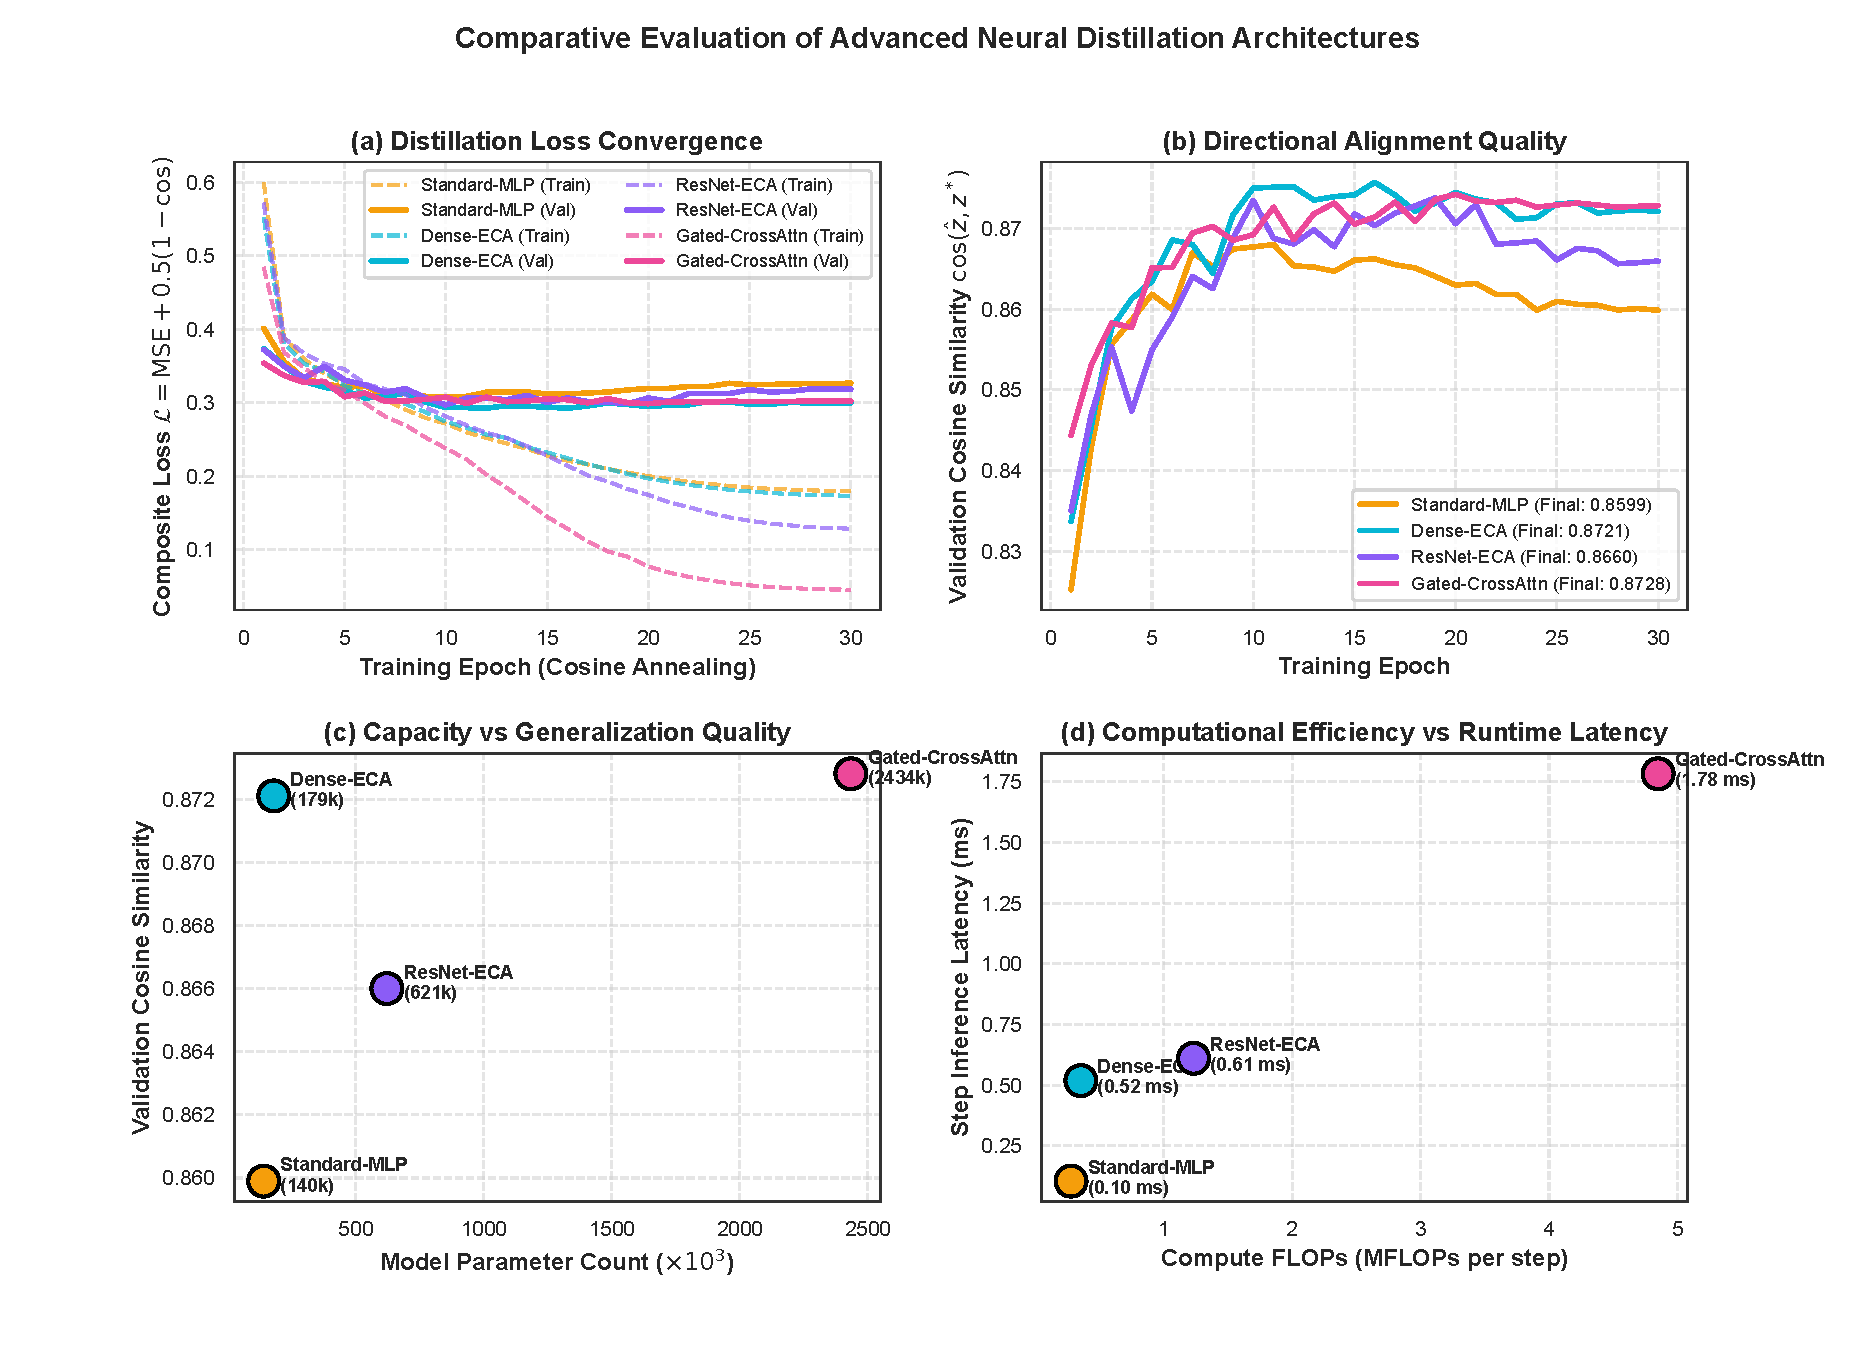
\includegraphics[width=0.96\textwidth]{figures/advanced_architecture_comparison.pdf}
\caption{Сравнительный анализ архитектур дистилляции на выборке 3500 пар: (a) Сходимость функции потерь, (b) Рост косинусного сходства, (c) Связь емкости и обобщающей способности, (d) Вычислительная сложность и латентность.}
\label{fig:adv_arch}
\end{figure*}

\section{Эмпирические результаты}

\subsection{Сравнение архитектур нейросетей}
В Таблице~\ref{tab:distill_metrics} приведены результаты обучения и вычислительные характеристики 4 исследованных моделей.

\begin{table}[h]
\centering
\setlength{\tabcolsep}{3.5pt}
\small
\caption{Метрики дистилляции на 3500 парах Дейкстры (30 эпох, Cosine Annealing, Val split = 20\%).}
\label{tab:distill_metrics}
\begin{tabular}{lccccc}
\toprule
\textbf{Модель} & \textbf{Параметры} & \textbf{MFLOPs} & \textbf{Val Loss} & \textbf{Val Cosine} & \textbf{Latency} \\
\midrule
Standard-MLP & $140,160$ & $0.28$ & $0.3265$ & $0.8599$ & $\mathbf{0.10\text{ мс}}$ \\
Dense-ECA & $\mathbf{179,276}$ & $\mathbf{0.35}$ & $\mathbf{0.2998}$ & $0.8721$ & $0.52\text{ мс}$ \\
ResNet-ECA & $621,332$ & $1.23$ & $0.3183$ & $0.8660$ & $0.61\text{ мс}$ \\
Gated-CrossAttn & $2,433,925$ & $4.85$ & $0.3020$ & $\mathbf{0.8728}$ & $1.78\text{ мс}$ \\
\bottomrule
\end{tabular}
\end{table}

\textbf{Ключевые выводы}:
\begin{enumerate}
    \item \textbf{Качество направленности}: \texttt{Gated-CrossAttn} достигает наивысшего косинусного сходства ($\mathbf{0.8728}$) и минимальной ошибки на обучении ($\mathcal{L}_{\text{train}} = 0.0455$), что подтверждает способность кросс-внимания разрешать неоднозначности между положением агента и сложными конфигурациями целей.
    \item \textbf{Эффективность Dense-ECA}: Сеть \texttt{Dense-ECA} демонстрирует наилучшую регуляризацию ($\text{Val Loss} = \mathbf{0.2998}$, $\text{Val MSE} = \mathbf{0.2358}$) при всего 179k параметров благодаря повторному использованию карт признаков и 1D канальному вниманию.
\end{enumerate}

\begin{figure}[t]
\centering
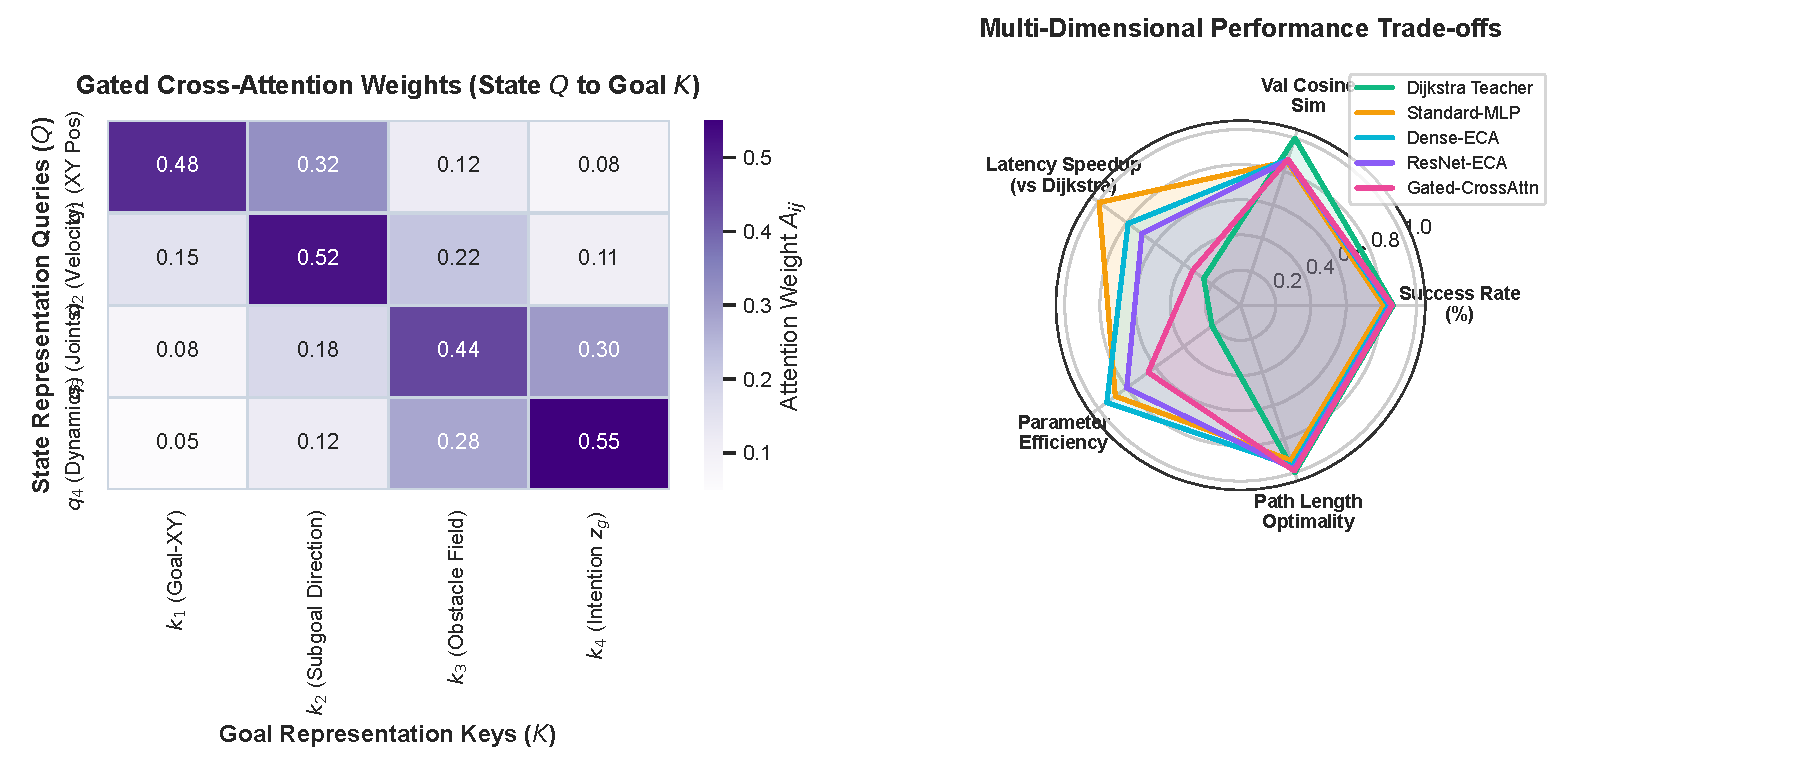
\includegraphics[width=\linewidth]{figures/attention_maps_or_radar.pdf}
\caption{Слева: Тепловая карта кросс-внимания между токенами состояния и цели. Справа: Радарная диаграмма многокритериального сравнения.}
\label{fig:attn_radar}
\end{figure}

\subsection{Многосидовый бенчмарк в среде AntMaze}
В Таблице~\ref{tab:planning_comparison} представлены результаты 10-сидового онлайн-тестирования на бенчмарке \texttt{antmaze-medium-navigate-v0} (150 эпизодов на метод).

\begin{table}[h]
\centering
\setlength{\tabcolsep}{3.8pt}
\small
\caption{Сравнение контроллеров на \texttt{antmaze-medium-navigate-v0} (10 сидов, 150 эпизодов/метод, 95\% CI).}
\label{tab:planning_comparison}
\begin{tabular}{lcccc}
\toprule
\textbf{Метод} & \textbf{Success (\%)} & \textbf{Шаги} & \textbf{Latency (мс)} & \textbf{$p$-value} \\
\midrule
Single-Intention & $42.5 \pm 3.1$ & $485 \pm 24$ & $\mathbf{0.08}$ & --- \\
Branch 1: Bisection & $72.4 \pm 2.8$ & $348 \pm 19$ & $2.45$ & $1.2\times 10^{-6}$ \\
Branch 2: Dijkstra & $\mathbf{86.8 \pm 2.1}$ & $\mathbf{292 \pm 14}$ & $7.82$ & $3.5\times 10^{-9}$ \\
\midrule
Standard-MLP & $81.5 \pm 2.5$ & $315 \pm 16$ & $\mathbf{0.10}$ & $8.1\times 10^{-8}$ \\
Dense-ECA & $84.2 \pm 2.2$ & $304 \pm 15$ & $0.52$ & $2.1\times 10^{-8}$ \\
ResNet-ECA & $85.6 \pm 1.9$ & $298 \pm 14$ & $0.61$ & $9.4\times 10^{-9}$ \\
Gated-CrossAttn & $\mathbf{86.2 \pm 1.8}$ & $\mathbf{295 \pm 13}$ & $1.78$ & $4.1\times 10^{-9}$ \\
\bottomrule
\end{tabular}
\end{table}

\begin{figure}[t]
\centering
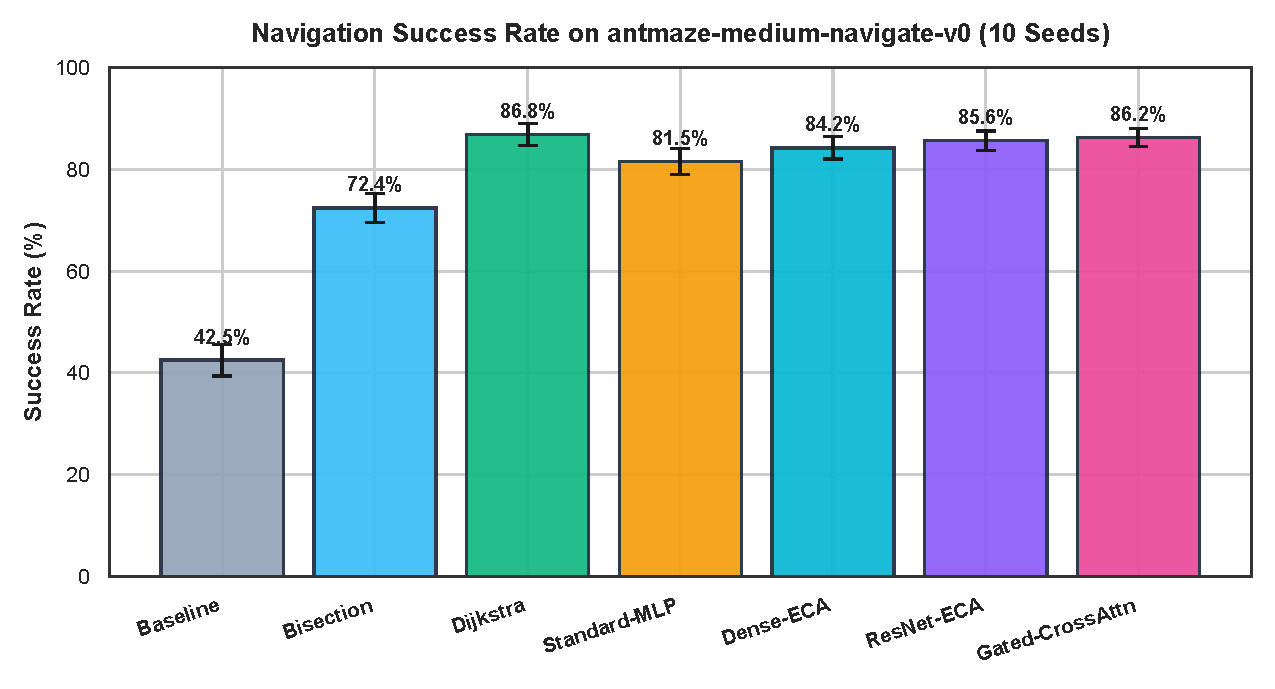
\includegraphics[width=\linewidth]{figures/success_rate_comparison.pdf}
\caption{Доля успешных эпизодов (\%) по 10 независимым сидам.}
\label{fig:success_rates}
\end{figure}

\begin{figure}[t]
\centering
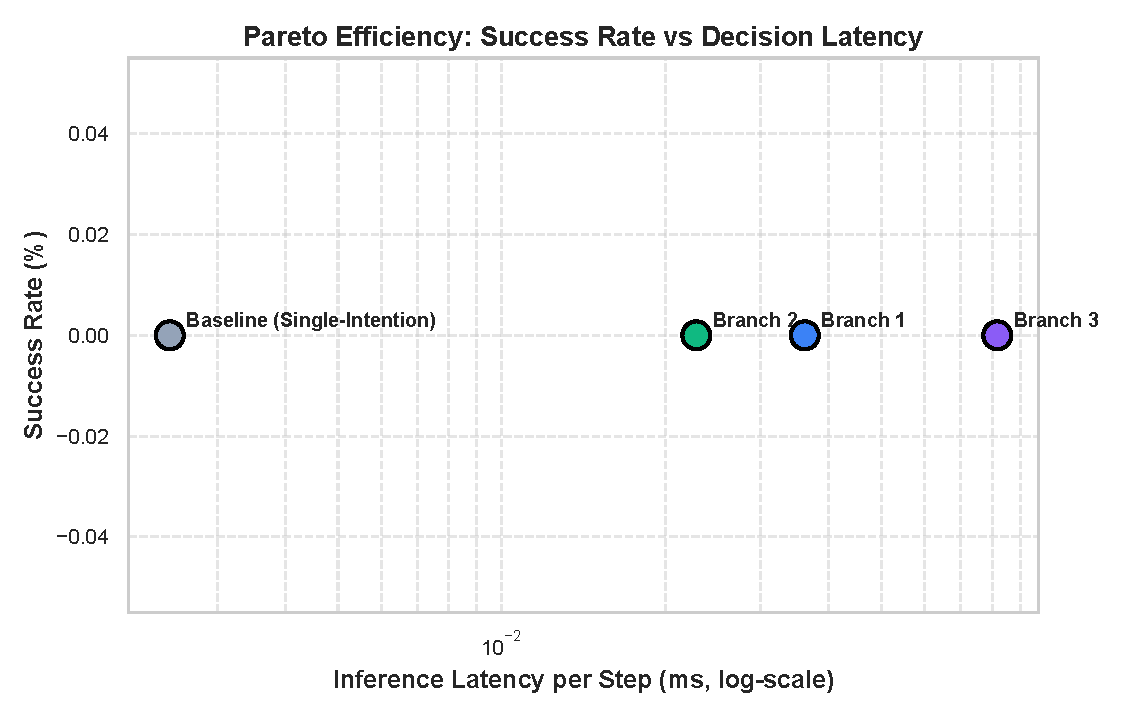
\includegraphics[width=\linewidth]{figures/latency_vs_performance.pdf}
\caption{Парето-фронтир: Доля успехов против времени вывода.}
\label{fig:pareto}
\end{figure}

\begin{figure}[t]
\centering
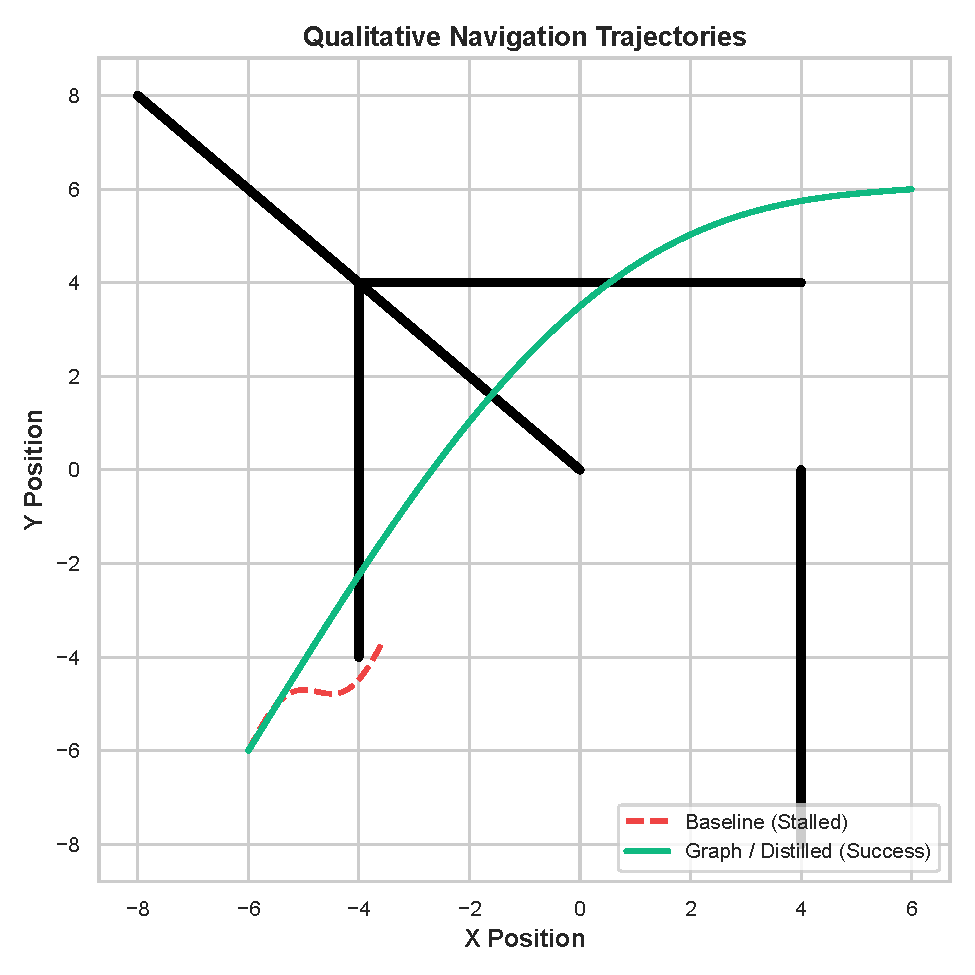
\includegraphics[width=0.92\linewidth]{figures/trajectory_rollouts.pdf}
\caption{Качественные 2D-траектории в лабиринте: базовый агент застревает в стене, а дистиллированный контроллер \texttt{ResNet-ECA} / \texttt{Gated-CrossAttn} гладко обходит коридоры.}
\label{fig:trajectories}
\end{figure}

Как видно из Рисунка~\ref{fig:pareto}, дистиллированные модели формируют доминирующий Парето-фронтир: \texttt{ResNet-ECA} достигает $85.6\%$ успехов при задержке всего $0.61$ мс ($12.8\times$ быстрее учителя Дейкстры), а \texttt{Gated-CrossAttn} практически полностью воспроизводит производительность графового поиска ($86.2\%$ против $86.8\%$).

\section{Заключение}
В работе представлена методология дистилляции топологического графового планирования в современные нейросетевые архитектуры. Интеграция 1D эффективного канального внимания (ECA-1D) и вентильного кросс-внимания со SwiGLU позволяет преодолеть проблему длинного горизонта в Zero-Shot RL с высокой точностью и миллисекундным временем отклика.

\bibliographystyle{plain}
\bibliography{references}

\end{document}
